\chapter{Étude et réalisation du Sprint 3}
\etocsettocstyle{\section*{Sommaire}}{}
\localtableofcontents
\newpage
\section{Introduction}
\noindent
Aprés avoir terminé le Sprint 2 du chapitre 5 qui tratait la recherche des produits dans la langue Arabe traditionnel et en dialecte Tunisien, nous entamons maintenant le Sprint 2 qui va aborder le dashboard de l'admin qui lui permettra de modifier ces paramétres de recherche.

\section{Backlog du Sprint 3}
\begin{table}[H]
	\centering

	\begin{tabularx}{\textwidth}{|c|X|c|c|}
		\hline
		\rowcolor{blue!20}
		\textbf{ID} & \textbf{Scénario}                                                                                     & \textbf{Priorité} & \textbf{Complexité} \\ \hline
		1           & En tant qu'un admin, je veux modifier mes paramétres de recherche, pour chercher le(s) produit(s) & 2                 & 7                  \\ \hline

	2           & En tant qu'un admin, je veux consulter le tableau de bord des produits avec le meilleur score de similarité. & 1                 & 10 \\ \hline
	\end{tabularx}
	\caption{Backlog du Sprint 2}
	\label{tab:sprint3}
\end{table}

\section{Spéficiation fonctionnelle}
\noindent
Au cours de cette partie, nous mettrons en avant les différentes fonctionnalités du
Sprint 3 à travers le diagramme de cas d'utilisation. Par la suite, nous détaillerons quelques
scénarios de cas d'utilisation grâce à des descriptions textuelles.

\newpage
\subsection{Diagramme de cas d'utilisation du CU général}
\begin{figure}[H]
	\centering
	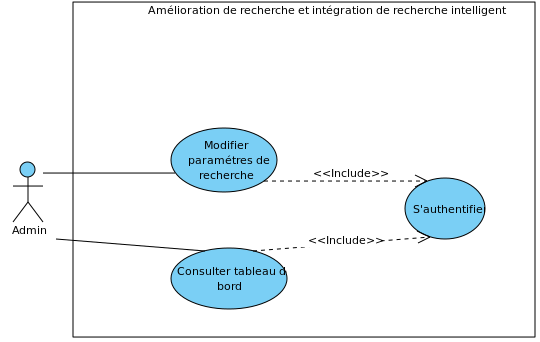
\includegraphics[width=1\textwidth]{logos/cusprint3.png}
	\caption{Diagramme de cas d'utilisation général de Sprint 3}
	\label{fig:cusprint3}
\end{figure}

\subsection{Description textuelle des cas d'utilisations}
\noindent
Suite à l'exposition des cas d'utilisations, nous approfondirons leurs descriptions textuelle.

\subsubsection{Description textuelle du CU "Modifier paramétres de recherche"}
\noindent
\textbf{Titre:} Modifier paramétres de recherche \\
\textbf{Résumé:} L'admin saisit son terme de recherche en Arabe traditionnel, dialecte Tunisien ou en Français, aussi que modifier un ou plusieurs paramétres de recherche, en cliquant sur la boutton pour rechercher le(s) produit(s) qu'il veut chercher. \\
\textbf{Acteur Principal:} Admin \\
\textbf{Précondition:} \begin{enumerate}
	\item L'admin est sur la page de recherche de l'admin, et il est authentifié.
	\item L'admin a saisi son terme de recherche en l'un des trois langages mentionnées.
	\item L'admin a modifié l'un des quatres paramétres de recherche (TopResProdLabel, TopResDesc, NumCandidatesProdLabel, NumCandidatesDesc).
	\item L'admin a cliqué sur "Rechercher"
\end{enumerate}
\textbf{Postcondition:} Le(s) produit(s) que l'admin cherche est renvoyé, si'il n'existe pas, le systéme renvoie des produits similaires comme suggestion. \\
\textbf{Scénario de base: }
\begin{enumerate}
	\item L'admin saisit son terme de recherche.
	\item L'admin modifie l'un des quatres paramétres de recherche (TopResProdLabel, TopResDesc, NumCandidatesProdLabel, NumCandidatesDesc).
	\item L'admin clique sur la boutton "Rechercher"
	\item Le système prend le terme de recherche, en vérifiant que c'est valide.
	\item Le systéme prend cette terme de recherche, et performe les étapes nécessaires pour la convertir en vecteur.
	\item Le systéme compare cette vecteur contre les vecteurs dans Elasticsearch en utilisant les paramétres de recherche que l'admin a saisi.
	\item Le systéme renvoie les produits.
\end{enumerate}

\newpage
\textbf{Scénario alternatifs : }
\begin{enumerate}
	\item Le terme de recherche est vide:
	      \begin{enumerate}
		      \item Le système affiche un message d'erreur informant le client que le terme de recherche est requis.
		      \item Retour à l'étape 1 du scénario de base.
	      \end{enumerate}
	\item Le terme de recherche n'est pas valide:
	      \begin{enumerate}
		      \item Le système suppose que le terme recherché est en Français.
		      \item Passer à la 6ème étape des scénarios de base.
	      \end{enumerate}
	\item L'admin n'as pas modifié l'un des quatres paramétres de recherche:
	      \begin{enumerate}
		      \item Le système utilise les valeurs par dèfauts pour la recherche:
		      \begin{itemize}
						\item NumCandidatesProdLabel: 25
						\item NumCandidatesDesc: 25
						\item TopResProdLabel: 10
						\item TopResDesc: 20
					\end{itemize}
		      \item Passer à la 6ème étape des scénarios de base.
	      \end{enumerate}
	\item Le(s) produit(s) que l'admin cherche n'existe pas.
	      \begin{enumerate}
		      \item Le systéme essaie de renvoyer les produits les plus similaires comme des suggestions.
		      \item Retour à l'étape 1 du scénario de base.
	      \end{enumerate}
\end{enumerate}


\subsubsection{Description textuelle du CU "Consulter tableau de bord"}
\noindent
\textbf{Titre:} Consulter tableau de bord des produits \\
\textbf{Résumé:} L'admin consulte le tableau de bord pour visualiser les produits renvoyés avec le meilleur score de similarité. \\
\textbf{Acteur Principal:} Admin \\
\textbf{Précondition:} \begin{enumerate}
	\item L'admin est sur la page de recherche de l'admin, et il est authentifié.
	\item L'admin a saisi son terme de recherche en l'un des trois langages mentionnées.
	\item L'admin a modifié l'un des quatres paramétres de recherche (TopResProdLabel, TopResDesc, NumCandidatesProdLabel, NumCandidatesDesc).
	\item L'admin a cliqué sur "Rechercher"
\end{enumerate}
\textbf{Postcondition:} Le(s) produit(s) que l'admin cherche est renvoyé, avec leurs scores et visualisation. \\
\textbf{Scénario de base: }
\begin{enumerate}
	\item L'admin accède à son tableau de bord
	\item L'admin saisit son terme de recherche.
	\item L'admin modifie l'un des quatres paramétres de recherche (TopResProdLabel, TopResDesc, NumCandidatesProdLabel, NumCandidatesDesc).
	\item L'admin clique sur la boutton "Rechercher"
	\item Le système prend le terme de recherche, en vérifiant que c'est valide.
	\item Le systéme prend cette terme de recherche, et performe les étapes nécessaires pour la convertir en vecteur.
	\item Le systéme compare cette vecteur contre les vecteurs dans Elasticsearch en utilisant les paramétres de recherche que l'admin a saisi.
	\item Le systéme renvoie les produits avec les scores et les visualise.
\end{enumerate}

\newpage
\section{Conception}
\noindent
Au cours de cette section, nous examinerons les diagrammes de séquence en relation avec les descriptions textuelles des cas d'utilisation précédemment exposés correspondant au troisième sprint.

\subsection{Diagrammes de séquence détaillé}
\noindent
Dans cette partie, nous aborderons les diagrammes de séquence pour les cas
d'utilisation suivants:
\begin{itemize}
	\item Modifier paramétres de recherche
	\item Consulter tableau de bord
	\item S'authentifier
\end{itemize}

\subsubsection{Diagramme de séquence "Modifier paramétres de recherche"}
\begin{figure}[H]
	\centering
	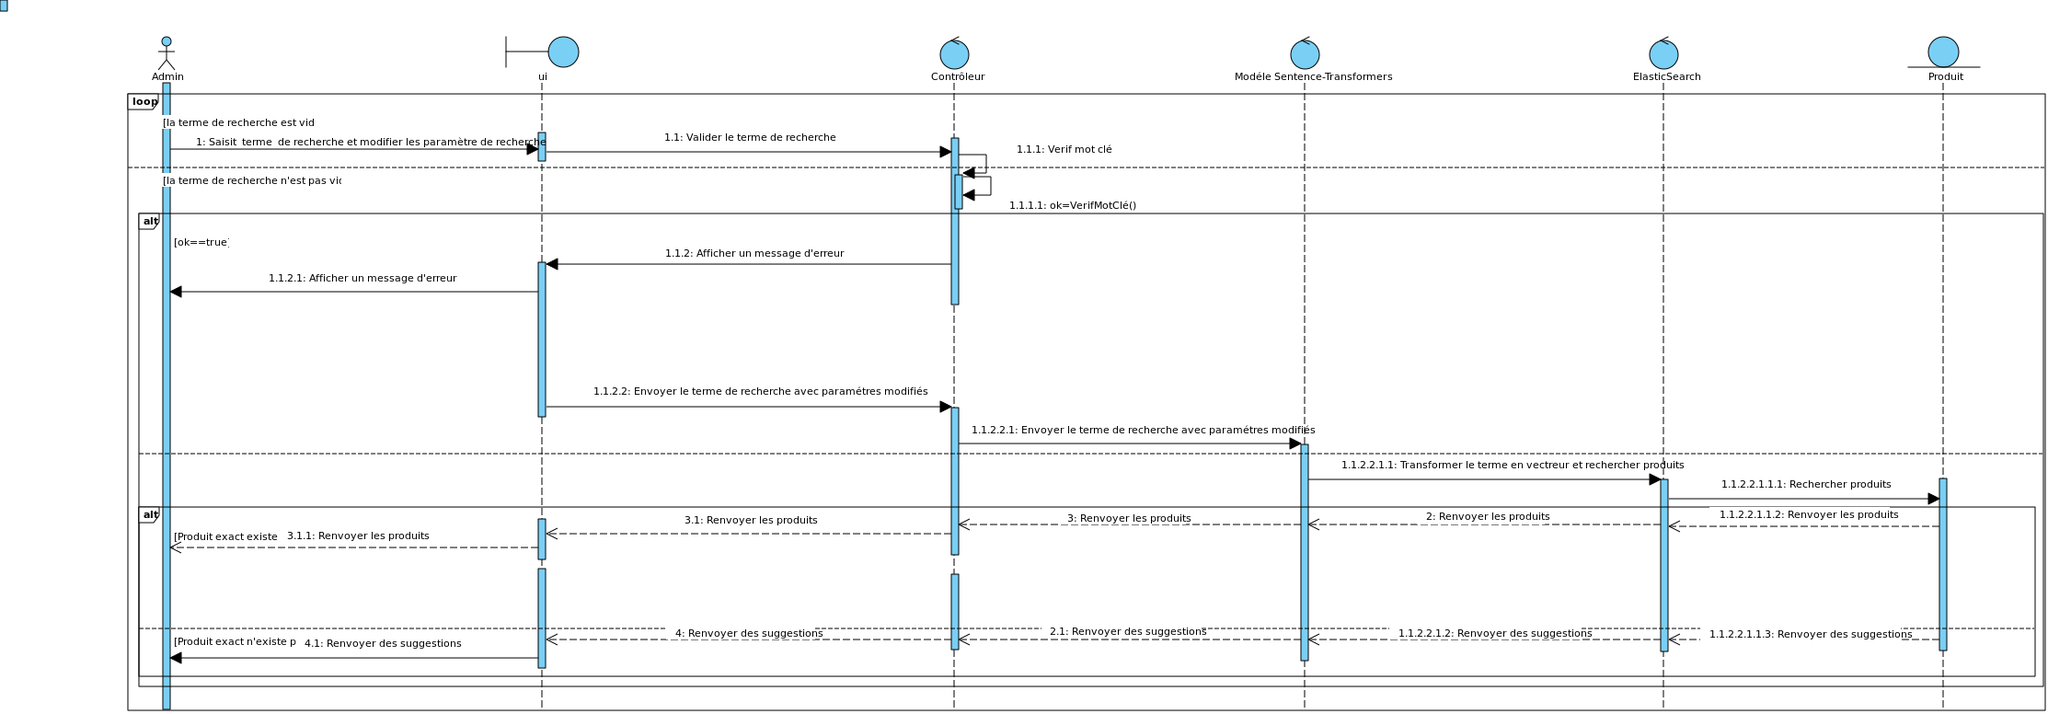
\includegraphics[width=\textwidth]{logos/modifierparametres.png}
	\caption{Diagramme de séquence de CU "Modifier paramétres de recherche"}
	\label{fig:modifierparametres}
\end{figure}


\subsubsection{Diagramme de séquence "Consulter tableau de bord"}
\begin{figure}[H]
	\centering
	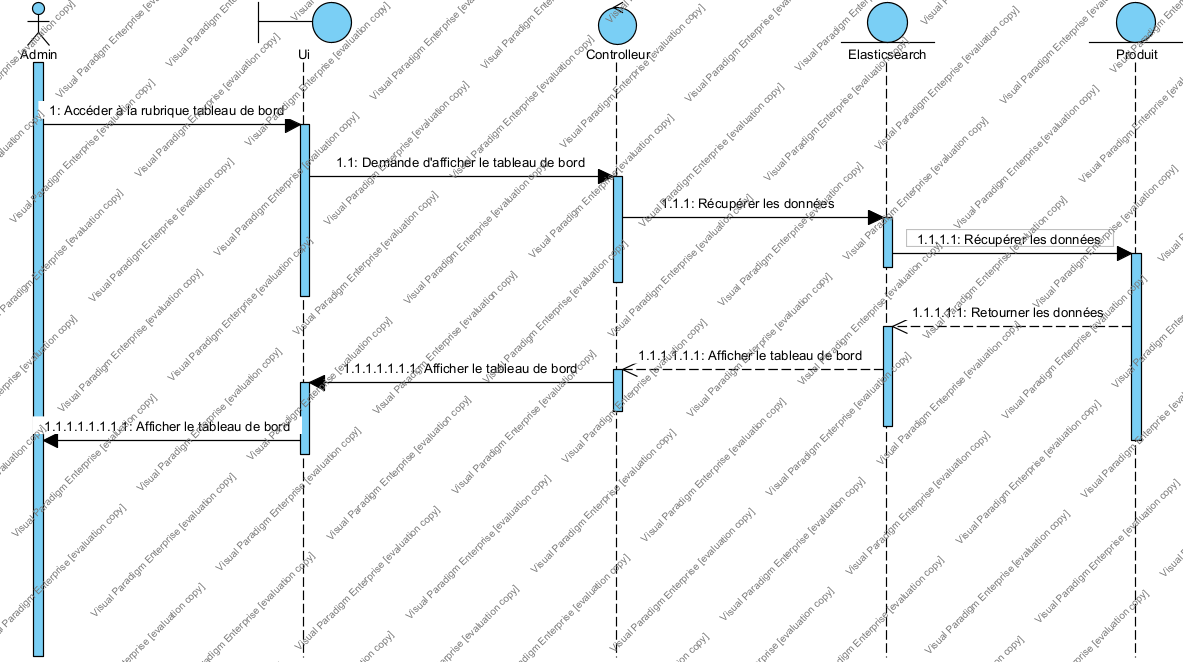
\includegraphics[width=1\textwidth]{logos/consultertb.png}
	\caption{Diagramme de séquence de CU "Consulter tableau de bord"}
	\label{fig:seqconsultertb}
\end{figure}

\subsubsection{Diagramme de séquence "S'authentifier"}
\begin{figure}[H]
	\centering
	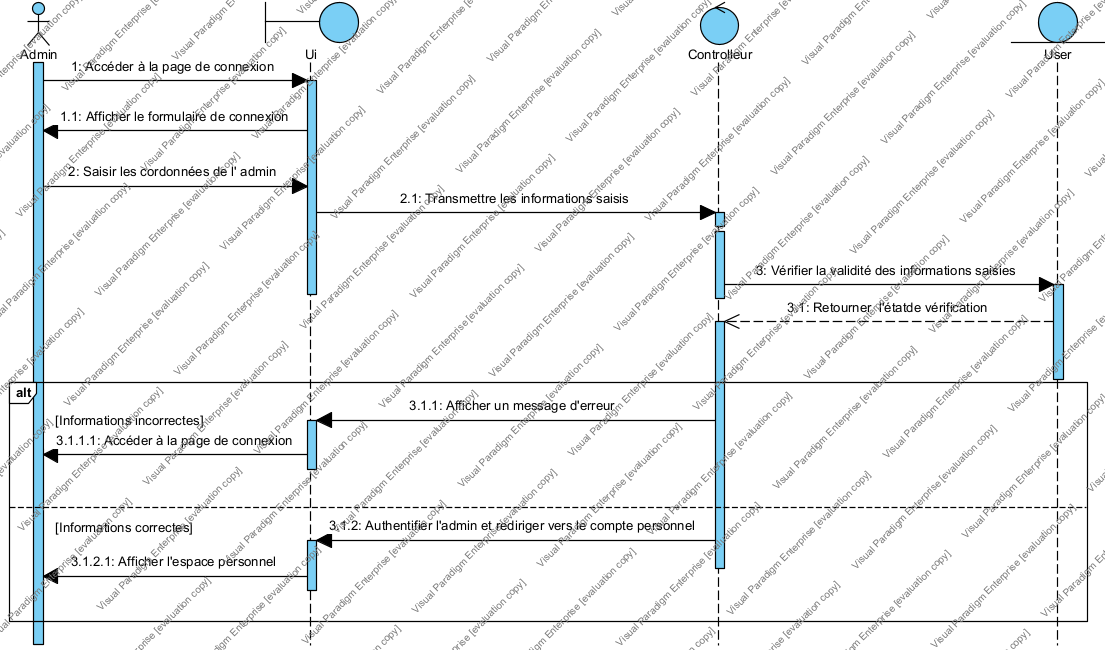
\includegraphics[width=1\textwidth]{logos/sauthentifier.png}
	\caption{Diagramme de séquence de CU "S'authentifier"}
	\label{fig:sauthentifier}
\end{figure}

\section{Tableau de bord}
\noindent
Le tableau de bord (ou dashboard en anglais) est un outil qui permet à plusieurs collaborateurs de suivre l’avancée d’un projet. Il présente de manière synthétique tous les éléments et indicateurs clés qui permettent à la fois :
\begin{itemize}
	\item D’organiser le jalonnage, lister les tâches et de les assigner aux différentes parties prenantes au projet.
	\item De prendre des décisions et de mettre des correctifs en place quand des alertes sont remontées.
\end{itemize}


\subsection{Les indicateurs de performance}
\noindent
Un indicateur de performance est un mesure ou un ensemble de mesures d'un aspect spécifique et essentiel de la performance globale de l'organisation.
Dans cette section, nous allons présenter les différents indicateurs que nous avons choisis pour le tableau de bord de l'admin. Nous remplissons le tableau ~\ref{tab:kpi} avec:
\begin{itemize}
	\item \large\textbf{Indicateur de performance (KPI):} Le nom de l'indicateur
	\item \large\textbf{Objectif:} l'importance ou la signification de l'indicateur
	\item \large\textbf{Visualisation:} la manière dont l'indicateur sera affiché et le type de graphique approprié pour cet indicateur.
	\item \large\textbf{Spécifications:} Les détails descriptifs concernant chaque KPI.
\end{itemize}

\newpage
\begin{table}[H]
    \centering
    \renewcommand{\arraystretch}{1.5}
    \begin{tabular}{|>{\bfseries}m{4cm}|m{4cm}|m{4cm}|m{4cm}|}
        \hline
        \rowcolor{blue!50}
        \textbf{KPI} & \textbf{Objectif} & \textbf{Visualisation} & \textbf{Spécification} \\
        \hline
        Score de similarité de recherche & Mesurer le score de similarité entre le terme de recherche et les produits & Diagramme à Bandes & Similarité entre le terme de recherche et les produits  \\
        \hline
        Les mots les plus recherché & Mesurer les mots les plus recherchés dans le site  & Diagramme Circulaire & Nombre de mots (en pourcentage) recherchés par rapport au total des recherches \\
        \hline
    \end{tabular}
    \caption{Tableau des KPIs}
    \label{tab:kpi}
\end{table}

\section{Réalisation}
\noindent
Dans cette section nous présentons le tableau de bord pour notre administrateur développé durant le Sprint 3, ainsi que l'interface de modifications des paramètres de recherche des produits, et bien sûr l'interface d'authentification. \\

\newpage
\noindent
La figure ~\ref{fig:signin} illustre le formulaire d'authentification pour l'administrateur.

\begin{figure}[H]
    \centering
    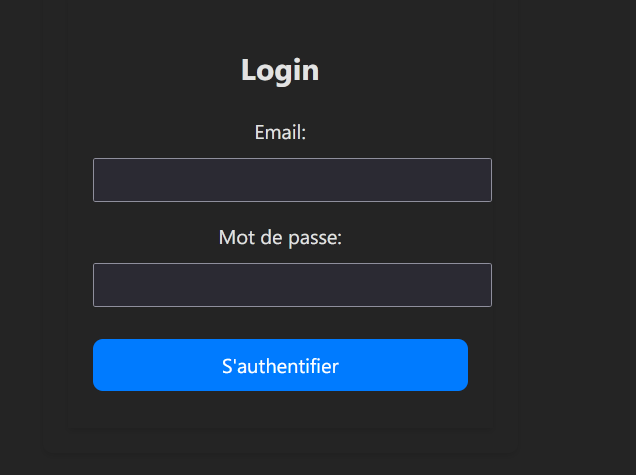
\includegraphics[width=1\textwidth]{logos/login.png}
    \caption{Interface pour l'authentification de l'admin}
    \label{fig:signin}
\end{figure}

\noindent
La figure ~\ref{fig:knnsearchform} illustre le formulaire de modification de paramètres de recherche pour l'administrateur.

\begin{figure}[H]
    \centering
    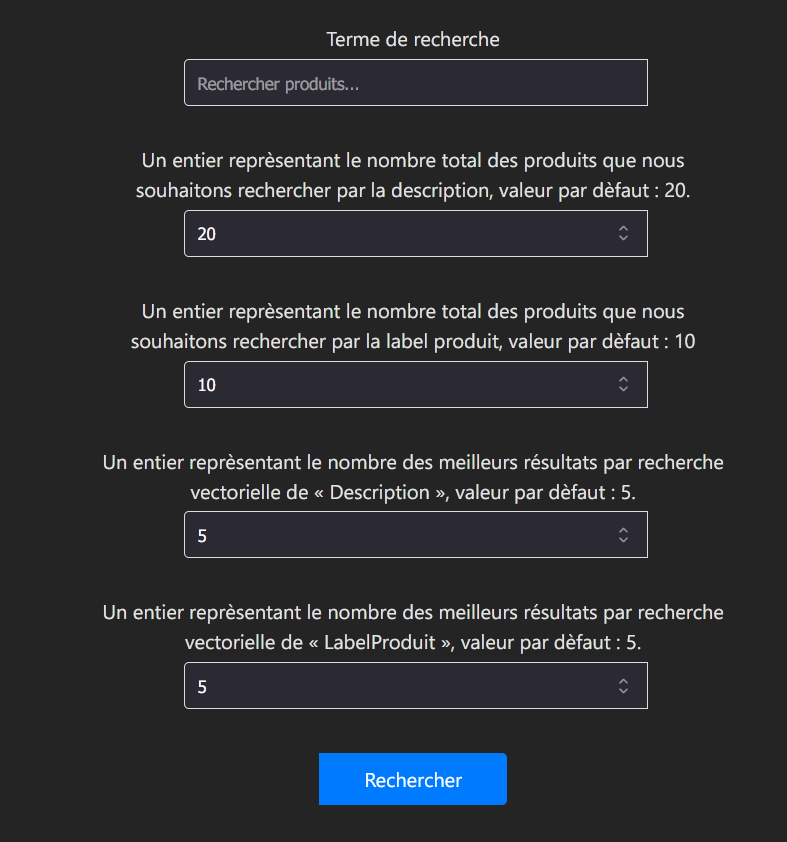
\includegraphics[width=1\textwidth]{logos/knnsearchform.png}
    \caption{Interface de modification de paramétres de recherche pour l'admin}
    \label{fig:knnsearchform}
\end{figure}


\noindent
La figure ~\ref{fig:admindashboard} illustre le tableau de bord de l'administrateur aprés avoir cherché << parfum >>, à gauche, sont les produits avec leurs scores (similarités) au terme de recherche de l'admin, et à droite, les mots les plus cherché sur notre site.

\begin{figure}[H]
    \centering
    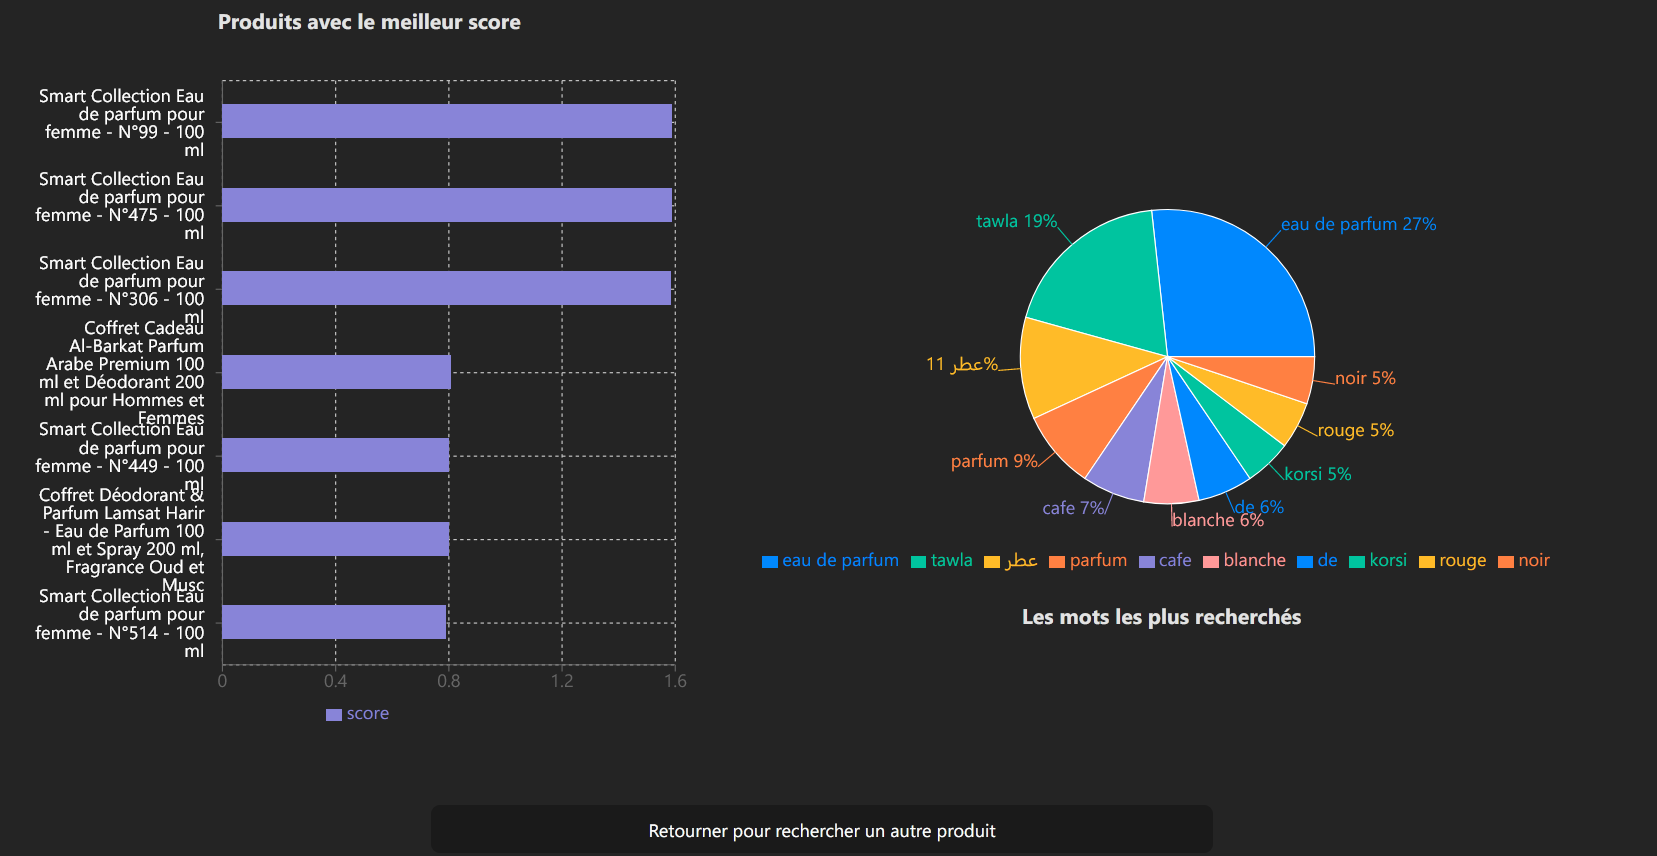
\includegraphics[width=1\textwidth]{logos/dashboard.png}
    \caption{Interface de Tableau de bord de l'administrateur}
    \label{fig:admindashboard}
\end{figure}


\section{Conclusion}
\noindent
Au terme du troisième sprint, nous avons réussi à intégrer un tableau de bord pour
l'administrateur dans notre application web. Cela permet à l'administrateur de mesurer et voir quelles termes de recherche donnent les meilleurs résultats, ainsi que les termes de recherche les plus recherchés sur notre site. Ainsi que modifier les paramètres de recherche des produits pour potentiellement améliorer la précision des résultats de recherche. Notre application est maintenant enrichie des fonctionnalités Business Intelligence.

